%%%%%%%%%%%%%%%%%%%%%%%%%%%%%%%%%%%%%%%%%%%%%%%%%%%%%%%%%%%%%%%%%%%%%%
% njuthesis 示例模板 v1.4.1 2024-04-19
% https://github.com/nju-lug/NJUThesis
%
% 贡献者
% Yu XIONG @atxy-blip   Yichen ZHAO @FengChendian
% Song GAO @myandeg     Chang MA @glatavento
% Yilun SUN @HermitSun  Yinfeng LIN @
% Yukai Chou @Muzimuzhi
%
% 许可证
% LaTeX Project Public License(版本 1.3c 或更高)
%%%%%%%%%%%%%%%%%%%%%%%%%%%%%%%%%%%%%%%%%%%%%%%%%%%%%%%%%%%%%%%%%%%%%%

%---------------------------------------------------------------------
% 一些提升使用体验的小技巧:
%   1. 请务必使用 UTF-8 编码编写和保存本文档
%   2. 请务必使用 XeLaTeX 或 LuaLaTeX 引擎进行编译
%   3. 不保证接口稳定,写作前一定要留意版本号
%   4. 以百分号(%)开头的内容为注释,可以随意删除
%---------------------------------------------------------------------

%---------------------------------------------------------------------
% 请先阅读使用手册:
% http://mirrors.ctan.org/macros/unicodetex/latex/njuthesis/njuthesis.pdf
%---------------------------------------------------------------------

\documentclass[
    % 模板选项(注意右端逗号):
    %
    % type = bachelor|master|doctor|postdoc, % 文档类型,默认为本科生
    % degree = academic|professional,        % 学位类型,默认为学术型
    %
    % nl-cover,   % 是否需要国家图书馆封面,默认关闭
    decl-page,  % 是否需要诚信承诺书或原创性声明,默认关闭
    %
    %   页面模式,详见手册说明
    % draft,                  % 开启草稿模式
    % anonymous,              % 开启盲审模式
    % minimal,                % 开启最小化模式
    %
    %   单双面模式,默认为适合印刷的双面模式
    % oneside,                % 单面模式,无空白页
    % twoside,                % 双面模式,每一章从奇数页开始
    %
    %   字体设置,不填写则自动调用系统预装字体,详见手册
    ,fontset = win, % |mac|macoffice|fandol|none,
  ]{njuthesis}

% 模板选项设置,包括个人信息、外观样式等
% 较为冗长且一般不需要反复修改,我们把它放在单独的文件里
\input{njuthesis-setup.def}

% 自行载入所需宏包
% \usepackage{subcaption} % 嵌套小幅图像,比 subfig 和 subfigure 更新更好
% \usepackage{siunitx} % 标准单位符号
% \usepackage{physics} % 物理百宝箱
% \usepackage[version=4]{mhchem} % 绘制分子式
% \usepackage{listings} % 展示代码
% \usepackage{algorithm,algorithmic} % 展示算法伪代码
\usepackage{listings}
\usepackage{float}
\usepackage[dvipsnames]{xcolor}
% 在导言区随意定制所需命令
% \DeclareMathOperator{\spn}{span}
% \NewDocumentCommand\mathbi{m}{\textbf{\em #1}}

\renewcommand{\lstlistingname}{代码}
\lstdefinestyle{pycharm}{
    language=Python,
    backgroundcolor=\color{white},
    basicstyle=\footnotesize\ttfamily,
    keywordstyle=\color{blue},
    stringstyle=\color{green!40!black},
    commentstyle=\color{gray}\emph,
    frame=single,
    numbers=left,
    numberstyle=\tiny\color{gray},
    captionpos=b,
    breaklines=true,
    breakatwhitespace=true,
    tabsize=4,
    showstringspaces=false,
    extendedchars=true,
    inputencoding=utf8,
    escapeinside={\%*}{*)},
}

% 开始编写论文
\begin{document}

%---------------------------------------------------------------------
%	封面、摘要、前言和目录
%---------------------------------------------------------------------

% 生成封面页
\maketitle

% 模板默认使用 \flushbottom,即底部平齐
% 效果更好,但可能出现 underfull \vbox 信息
% 以下命令用于抑制这些信息
\raggedbottom

\begin{abstract}
文言文作为中国传统文化的重要组成部分,把文言文保护好、传承好、发展好是传承中华文化的不可或缺的一部分。但由于文言文本身具有的复杂语法、与现代汉语的巨大差异,大大提高了文言文阅读的门槛、阻塞了文言文推广的进度,因此,充分发挥大语言模型在文本翻译领域的优势、构建文言文-现代文翻译模型、降低文言文阅读门槛是传承中华文化、加强中华民族凝聚力、实现中华文化现代化的重要关节。

本研究基于ChatGLM3-6B模型和Erya数据集,旨在设计和训练一种文言文到现代文的大语言翻译模型。通过对ChatGLM3-6B模型进行微调,并结合Erya数据集中的文言文和现代文平行语料,致力于提高模型在古代文献翻译任务中的性能。文章首先分析了当下主流开源预训练模型的特点和优劣,然后探究了微调方法的选择、评价指标的应用,并在训练集上进行了模型性能的比较分析。实验结果表明,我们设计的翻译模型在文言文到现代文的翻译任务中取得了良好的性能,相比百度翻译,在Rouge分数上取得了平均+5Rouge的优势;与【随无涯】翻译模型相比,取得了+7Bleu、平均+10Rouge的进步;与mengzi-t5-base模型相比,在Bleu-4和Rouge-2上有+3Bleu、+8Rouge-2的改进,为古代文献研究和相关应用提供了有力支持。

\end{abstract}

\begin{abstract*}
As an important part of traditional Chinese culture, the protection, inheritance, and development of Classical Chinese are indispensable for the inheritance of Chinese culture. However, due to the complex grammar and significant differences from modern Chinese, Classical Chinese greatly increases the threshold for reading and hinders the promotion of Classical Chinese. Therefore, fully leveraging the advantages of large language models in the field of text translation, constructing Classical Chinese to Modern Chinese translation models, and reducing the threshold for Classical Chinese reading are crucial for the inheritance and modernization of Chinese culture, as well as strengthening the cohesion of the Chinese nation.

This study aims to design and train a Large Language Model for translating Classical Chinese to Modern Chinese based on the ChatGLM3-6B model and the Erya dataset. By fine-tuning the ChatGLM3-6B model and combining Classical Chinese and Modern Chinese parallel corpora from the Erya dataset, we strive to improve the performance of the model in translating ancient texts. In this thesis, we first analyze the characteristics and advantages and disadvantages of mainstream open-source pre-trained models, then explore the selection of fine-tuning methods and the application of evaluation metrics, and finally compare and analyze the performance of the model on the training set. The experimental results demonstrate that our designed translation model performs well in translating Classical Chinese to Modern Chinese. Compared to Baidu Translate, our model achieves an average advantage of +5 Rouge scores. Compared to the 【Sui Wuya】 translation model, it shows an improvement of +7 Bleu and an average of +10 Rouge scores. Additionally, compared to the mengzi-t5-base model, our model improves by +3 Bleu and +8 Rouge-2 scores in Bleu-4 and Rouge-2, providing strong support for the study of ancient literature and related applications.
\end{abstract*}

% 生成目录
\tableofcontents
% 生成图片清单
\listoffigures
% 生成表格清单
\listoftables

%---------------------------------------------------------------------
%	正文部分
%---------------------------------------------------------------------
\mainmatter

% 符号表
% 语法与 description 环境一致
% 两个可选参数依次为说明区域宽度、符号区域宽度
% 带星号的符号表(notation*)不会插入目录
% \begin{notation}[10cm]
%   \item[DFT] 密度泛函理论 (Density functional theory)
%   \item[DMRG] 密度矩阵重正化群 (Density-Matrix Reformation-Group)
% \end{notation}

% 建议将论文内容拆分为多个文件
% 即新建一个 chapters 文件夹
% 把每一章的内容单独放入一个 .tex 文件
% 然后在这里用 \include 导入,例如
%   \include{chapters/introduction}
%   \include{chapters/environments}

\chapter{引言}

\section{研究背景及意义}

2022年4月,中共中央办公厅、国务院办公厅发表《关于推进新时代古籍工作的意见》,强调要做好古籍保护、传承、发展工作,维护和弘扬好祖国宝贵文化遗产\cite{XYDU202403001}。中华文化的现代化是延续优秀传统文化的现代化而不是消灭传统文化的现代化,文言文作为中国传统文化的重要组成部分,推广和传承文言文更是传承中华文化、加强中华民族凝聚力、实现中华文化现代化的重要关节。而局限于文言文的语法和现代文之间的区别,其翻译一直是一个具有挑战性的任务,这大大限制了现代人对文言文的阅读和理解文言文美学的能力。

因此,建立文言文翻译工具具有重要的学术和应用价值。首先,文言文翻译系工具作为文言文学习者的一个稳定、准确的学习工具,帮助其更好地理解和掌握文言文的语法和写作方式,从而降低学习难度。通过与工具互动,学习者能够翻译、分析文言文文本,获取语言知识和文化背景,提升阅读能力和文言文水平。其次,该工具对文言文研究和保护至关重要,为研究人员提供高质量的翻译服务,帮助他们更好地理解和分析文言文文献,挖掘知识和价值。最后,自动化翻译方式大幅提高了翻译效率,为文言文研究提供更多资源和工具支持。

然而,传统机器翻译方法在文言文-现代文翻译任务中面临着句法结构复杂、典故丰富和词汇特殊等挑战,导致翻译质量不尽如人意。近年来,随着人工智能的快速发展,特别是在自然语言处理和机器学习领域,大型语言模型(如GPT系列)通过深度学习和海量数据训练,具有较强的语言理解能力和文本生成能力,在文本翻译、文本生成、聊天机器人等多个任务中取得了显著的效果。基于这些人工智能大型语言模型的文言文翻译系统也显示出巨大的潜力,能够通过学习大量文言文语料,自动捕捉文言文的语法规则、词义和文化背景,实现更准确、流畅的翻译。

采用人工智能大语言模型构建的文言文翻译系统还有助于推动人工智能研究和技术发展。通过解决文言文翻译中的挑战,如复杂的语法结构和文化理解,可以推动大模型在其他自然语言处理任务中的应用,并改进其训练和应用方法,提升性能和可扩展性。

综上所述,构建文言文翻译系统具有重要学术、应用和技术价值,为文言文学习、研究和保护提供了强大支持,促进了中外文化交流与理解,同时推动了人工智能研究和发展的进步。

\section{国内外研究现状}
在21世纪初期,语言模型的实现主要依赖统计方法,通过统计词语序列等方法来估计其概率分布,这些模型结构较为简单,在机器翻译领域取得了一定成果,为后续的技术发展奠定了基础。

自从Yoshua Bengio教授提出通过神经网络解决语言模型问题之后\cite{bengio2000neural},语言模型的探索便进入了神经网络时代,人们开始探寻通过神经网络建模语言的方法,到21世纪10年代初期,RNN(循环神经网络)\cite{mikolov2010recurrent}已经被广泛应用于语言建模任务,其能够捕捉语言文本输入序列中的依赖关系。随后,LSRTM(长期记忆网络)\cite{hochreiter1997long}的提出更是进一步解决了RNN难以处理长序列数据的问题,解决了语言模型在面对长文本是难以记忆长期依赖信息的问题。

2017年,Google Brain团队提出的Transformers模型\cite{vaswani2017attention}彻底改变了语言模型领域的格局,Transformers通过构建基于自注意力机制的神经网络,能够进行并行计算并且有效的捕捉长距离的依赖关系。Transformers的出现摈弃了传统的循环神经网络和卷积神经网络,彻底改变了语言模型的建模方式,大幅提升了训练速度和性能,使得语言模型在计算效率和模型表现上取得了显著提升。

Google于2018年发布了BERT模型\cite{devlin2018bert},BERT模型是在Transformer架构上进行改进和扩展的预训练模型通过上下文编码器,能够更好的理解和展现文本预警。同时,BERT模型通过无监督预训练和有监督微调下游任务的方式,实现了同一种模型在多种自然语言处理任务上的优秀表现,标志着大规模预训练模型的兴起。

OpenAI发布的GPT系列模型也是大语言模型发展过程中极重要的一环,其于2018年发布的采用单向自回归预训练方式的GPT-1模型\cite{radford2018improving}展现了GPT预训练模型在NLP领域的巨大潜力。随后OpenAI于2019年发布的GPT-2模型\cite{radford2019language}在GPT-1的基础上进一步使用了更大规模的预训练数据和更深层次结构的神经网络,并去掉了fine-tune层,不再需要定义模型具体的下游任务。而2020年出现的GPT-3模型\cite{brown2020language}更是达到了1750亿个参数的超大规模,在广泛的NLP任务,如文本生成、文本分类、文本翻译上取得了令人惊讶的成绩。OpenAI的GPT模型,及其发布的chatGPT聊天机器人在展示大规模预训练模型在自然语言处理任务中的卓越表现、推动预训练模型技术的发展的同时,也证明了大语言模型迅速走向民用、步入商业化的可行性,大大加速了大语言模型商业化、规模化的进程。

而Google于2020年发布的T5模型\cite{raffel2020exploring}提出将所有的语言建模任务都视为text-to-text的的问题,这样就可以实现通过同一个模型、目标函数、解码器来解决不同的下游NLP任务,大大提高了大语言模型的灵活性。

随着大语言模型技术的迅速发展,国内企业和高校也推出了众多国产大语言模型。比较著名的有阿里云团队于2023年前后陆续发布Qwen综合的言模型系列\cite{bai2023qwen},目前共发布包括1.8B、7B、14B等具有不同参数量的一系列模型。以及清华提出的一种基于自回归空白填充的通用语言模型(GLM)\cite{du2021glm},通过改进空白填充预训练,在NLU、条件生成和无条件生成的广泛任务中取得了优于BERT、T5和GPT的表现,证明了其对不同下游任务的泛化能力,并让清华技术成果转化的公司智谱AI依据GLM发布开源预训练大模型ChatGLM,推进国内大语言模型的开源和商用进展。

现阶段大语言模型的主流应用方式就是依托第三方开源的预训练大语言模型,根据需要的下游任务构建自己的数据集并进行微调,本项目就是使用于清华发布的GLM系列模型ChatGLM3-6B使用P-tuning v2方法\cite{liu2021p}进行下游任务的微调。

\section{文言文翻译的难点}
现有的语言翻译模型层出不穷,但是主流的翻译模型大多是针对大语种的翻译模型,尤其以英语对其他语言的翻译为主,而文言文-现代文这种小语种翻译的研究则比较少。同时文言文翻译本身具有以下难点:
\begin{itemize}
    \item 文言文的语法结构与现代汉语有很大不同。文言文通常采用简洁精炼的句式,省略主语和谓语的情况较多,句子结构松散且灵活。而现代汉语则更加注重完整的句式和明确的语法规则。这种结构上的差异使得直接转换常常导致语义不清或表达不完整,翻译模型无法获取足够的上下文信息,对文本语义的理解不够。
    \item 文言文中的词汇相对于现代汉语更加古朴和精炼,且很多词语在现代汉语中已经不再使用或意思发生了变化。例如,文言文中的“夫”、“其”、“者”等虚词在现代汉语中使用频率较低且意义有所不同。此外,文言文中常用的典故、成语和修辞手法,也增加了翻译的难度,需要对其进行准确理解和适当转换。
    \item 文言文的表达方式往往非常灵活和富有创造性,同时文言文本身高度要求文本的优雅性和文学性,这导致同一句文言文可能有多种不同的现代汉语翻译版本,这要求翻译模型不仅要能够准确理解原文,还要具备一定的翻译创造力,选择最优雅的现代汉语表达方式,这对于机器翻译模型来说是一个巨大的挑战。
    \item 文言文通常包含丰富的历史、文化和哲学背景,在人工翻译时就要求译者具备深厚的文化知识和历史背景,才能准确理解和翻译其中的内容。在输入翻译模型时就更要求模型对文言文语义的理解更加深刻,对模型的理解能力提出了更高的要求。
\end{itemize}

\section{研究内容与主要工作}
本项目主要工作是基于公司或企业发布的开源预训练大语言模型,输入构建的文言文原文-现代文翻译平行语料数据进行微调训练获得针对文言文翻译的大语言模型,主要工作如下:
\begin{itemize}
    \item 收集并分析当下的主流大语言模型,并分析他们的优缺点。我们收集了当下主流的一些开源预训练大语言模型,梳理了大语言模型的发展过程,分析了这些模型的结构特点、性能倾向和各自的优势下游任务,
    \item 整理并提出一个用于微调大语言模型的文言文-现代文平行语料数据集。针对文言文翻译任务中,文言文-现代文语料数据集稀少、现有数据集质量层次不齐的问题,我们收集了多个现有的文言文-现代文语料数据集,通过脚本对这些数据集中的数据进行清洗,构建不同数据规模的数据集,获得了高质量的文言文-现代文语料数据集。
    \item 将提出的数据集用于开源预训练模型的微调,并与其他模型在测试集上比较性能的差异。我们将构建的高质量的文言文-现代文语料数据集用于基线模型ChatGLM3-6B的微调训练,让模型适应在文言文翻译这一下游任务,打破了基于Transformers、BERT等国外开源模型构建翻译模型的传统,使用对中文语境有更强的适应性国产开源大语言模型,让模型在文言文翻译任务上具有更好的性能。
\end{itemize}

\section{论文组织结构}
本文主要介绍了当前大语言模型的发展状况,构造了一个文言文-现代文平行语料数据集,通过数据集对大语言模型进行微调,并分析不同模型、不同参数、不同规模数据集之间的差异,确定一个性能最佳的翻译模型,并最终与现有的一些主流翻译模型/软件进行对比实验。

第一章:引言。主要介绍了目前大语言模型的发展现状、背景和应用方法,介绍了项目的主要任务和论文的结构。

第二章:基本概念和相关工作。主要介绍了当下主流的几个大语言模型的结构、原理和优缺点,分析了几个主流国产开源预训练模型的特点。

第三章:大语言模型微调实验设计。具体描述了微调实验的数据集构建、微调的训练、以及介绍了实验所使用的微调方法,并分析了模型在训练过程中性能的变化。

第四章:实验结果及分析。介绍了微调模型对比实验的设计和细节,对比分析了不同参数设置下微调模型的性能差异。

第五章:总结与展望。分析了本次实验的缺陷和问题,提出一些针对实验的可能的改进方法以及未来后续任务的展望。


\chapter{基本概念和相关工作}

\section{大语言模型介绍}
\subsection{大语言模型}
大语言模型(Large Language Model)是一种基于神经网络的NLP技术,可以通过学习自然语言的范式和规律执行处理任务,其最主要特征就是“大”,即参数规模庞大、能处理大量语言数据、具有强大理解能力。大语言模型的基本思想是通过将NLP任务中的自然语言文本看作一段输入序列,即文本序列或向量序列,模型内部的神经网络可以处理这些序列来生成对应的输出序列。

相比之前NLP领域的技术,依托庞大的参数规模,大语言模型具有更好的理解能力和学习能力,从而在下游任务中获得更好的性能。同时大语言模型强调端到端的学习方法,直接从构建的初始文本数据中进行学习,避免了传统方法中需要人工设计特征或规则的复杂方法。也由于庞大的参数规模,大语言模型训练的资源消耗量大、对数据依赖性强,以及在面对从未见过的数据时泛化能力不足。

\subsection{Transformers}
Transformers于2017年被第一次提出\cite{vaswani2017attention},是一种处理序列数据的深度学习模型。Transformers的模型结构如图\ref{Transformers}所示,是一种典型的编码器-解码器结构模型,编码器部分将输入的文本序列编码成向量,解码器部分针对该向量编码进行解码获得作为输出的文本序列。经过训练的编码器-解码器结构模型可以从输入文本序列生成输出文本序列。

\begin{figure}[ht]
  \centering
  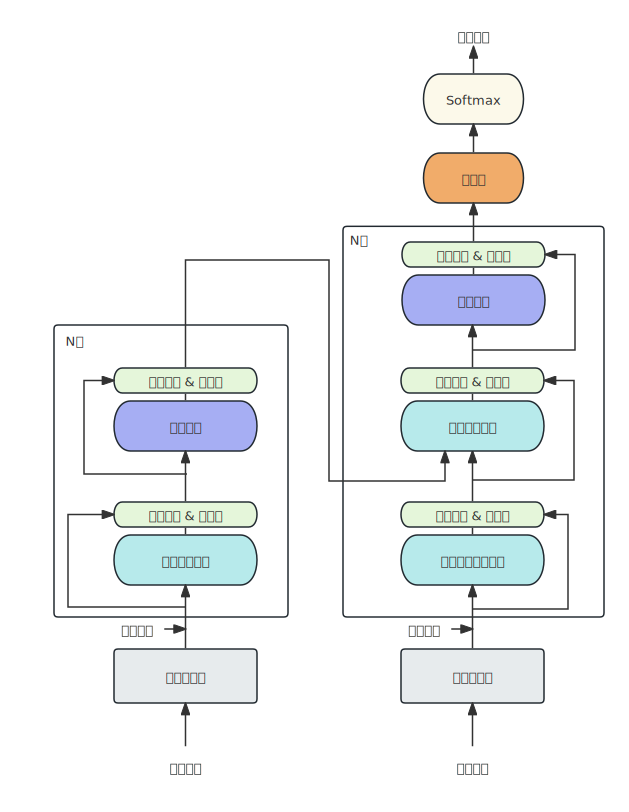
\includegraphics[width=0.85\textwidth]{image/transformers.pdf}
  \caption{Transformers的模型结构}
  \label{Transformers}
\end{figure}

最初的Transformers结构中,模型的编码器和解码器均是由6个相同的子层组成的,编码器的每个子层由一个前馈网络和一个多头注意力层构成,解码器的子层则多一个掩码多头注意力层,通过注意力层建立序列内部的关联性、通过前馈网络对每个位置编码的隐藏表示进行变换和映射,之后每个子层连接到一个残差连接和归一化层。在解码器末端通过线性层将输出向量映射到词汇表上,在通过Softmax函数归一化,得到最终的输出概率分布。

Transformers相比之前的语言模型的最大优势就是Transformers能够迅速适应不同的下游任务,从业者只需要在预训练模型的基础上使用自己的小规模数据集对其进行调整就可以让模型适应新的任务。

% \subsection{BERT}
% BERT是基于Transformers的编码器架构的语言模型\cite{devlin2018bert},核心思想是多层编码器堆叠,因此BERT本身只应用于输入文本序列的编码而不输出文本。BERT引入了两种训练任务:遮蔽语言模型(MLM)和下一句预测(NSP),来进行无监督的预训练。BERT通过遮蔽语言模型来随机遮掩输入序列中的一部分标记,让模型通过其余标记来预测被遮掩的标记,使模型能学习到双向的语言表示关系。下一句预测任务旨在判断两个句子是否是连续的,使模型捕捉到句子之间的关联性,理解句子之间的语义关系。

% BERT模型的优势在于其是第一个引入双向上下文的模型,解决了以往模型只能单向或浅双向的问题,具有革命性的突破意义。同时BERT是完全的无监督训练,因此可以在更庞大、更原始的纯文本语料库上进行训练和微调。

% \subsection{GPT}
% GPT(Generative Pre-trained Transformer)\cite{radford2018improving}是由OpenAI提出的预训练模型,也是一种基于Transformers架构的模型。与BERT相反,GPT模型结构是由多个相同的Transformers解码器堆叠而成的,每个解码器包括多个自注意力层和前馈网络。GPT使用了单向注意力机制,模型在生成当前位置的词语时只关注前面已有的词语,因此GPT在文本生成上更符合自然语言的生成顺序,同时由于其解码器堆叠而成的结构,GPT模型在文本生成任务上有显著的优势。

% GPT模型的独特之处在于其训练方法是一种半监督的训练方法,致力于使用大量无标注的数据对模型进行预训练,让模型学会普遍的“常识”,之后再使用有标注的数据对模型进行微调,实现模型对下游具体任务的适配,图\ref{GPT}展示了GPT如何在不改动模型结构的情况下适配不同的下游任务。

% \begin{figure}[ht]
%   \centering
%   \includegraphics[width=\textwidth]{image/GPT.pdf}
%   \caption{GPT的结构,上半部为12层的Transformers的解码器结构,下半部展示了GPT通过将不同任务的输入序列进行组合来适配下游任务}
%   \label{GPT}
% \end{figure}

\subsection{T5}
T5是由Google提出的基于Transformers的编码器-解码器结构的模型\cite{raffel2020exploring},和以往不同的是,T5统一了输入和输出的表现形式,预训练模型不再需要使用特定的数据集针对具体的下游任务进行有监督的微调。T5模型将所有的NLP任务都看作text-to-text的任务,将不同下游任务的输入转化为几乎一致的格式,即“任务前缀声明+输入文本”。因此,在T5模型上不在有文本生成、文本摘要、文本翻译等细分的下游任务,也就做到了通过一套损失函数、评估指标等来评测不同任务,也可以方便的评估模型结构、数据集、损失函数对不同任务的影响。

% \subsection{M2M-100}
% M2M-100模型是由FaceBook发布的基于Transformers架构的翻译模型\cite{fan2021beyond},与以往的翻译模型不同,M2M-100不仅实现了多种语言之间互相翻译,而且可以进行直接翻译而不经过中间语言,实现了“多对多”的翻译模式。

% 如图\ref{M2M100}所示,M2M-100通过让编码器和解码器在不同语言之间共享参数来实现在不同语言之间统一表示空间和参数,使得模型在多对多语言翻译任务中不需要一个中间语言作为过渡,可以同时处理多种语言的翻译任务。

% \begin{figure}[ht]
%   \centering
%   \includegraphics[width=\textwidth]{image/M2M-100.pdf}
%   \caption{M2M100通过特定的语种参数直接在两种语言之间进行翻译}
%   \label{M2M100}
% \end{figure}

\section{国产开源预训练大语言模型}
\subsection{Qwen}
Qwen是由阿里旗下通义千文发布的一系列大语言模型,包括基础预训练语言模型(基座模型)、聊天模型(Qwen-Chat)、编码专用模型(Code-Qwen)、数学专用模型(Math-Qwen-Chat)等多个版本,以满足不同需求的应用,适用于各种应用场景和下游任务。Qwen-Chat模型使用人类反馈强化学习训练(RLHF)\cite{christiano2017deep},具有先进的对话生成能力,展现出优秀的工具使用和规划能力。编码专用模型和数学专用模型,如Code-Qwen和Math-Qwen-Chat为编程和数学领域的语言理解提供了更专业的支持,Qwen系列模型汇总如图\ref{Qwen}所示。

\begin{figure}[ht]
  \centering
  \includegraphics[width=\textwidth]{image/Qwen.pdf}
  \caption{Qwen系列模型脉络}
  \label{Qwen}
\end{figure}

Qwen采用了改进版的Transformer架构,并使用LLaMA\cite{touvron2023llama}的训练方法,并做出了以下改进:
\begin{itemize}
    \item 嵌入和输出映射不共享权重,从而以内存开销为代价获得更好的性能。
    \item 使用了RoPE(旋转位置编码)\cite{su2024roformer}进行位置编码,因为需要优先考虑模型性能以及追求较高的精度,并放弃BF16和FP16转而采用了FP32精度的逆频率矩阵。
    \item 使用了预归一化(Pre-Norm)和RMSNorm进行规范化,与后归一化相比,已被证明能提高训练的稳定性。
    \item 使用了SwiGLU作为激活函数,它是Swish和Gated Linear Unit的组合。
    \item 除了在QKV(查询、键、值)层中保留Bias以外,在大多数层中都移除了Bias,以提高模型的外推能力。
\end{itemize}

目前Qwen已经发布Qwen-1.8B、Qwen-7B、Qwen-14B、Qwen-72B等预训练模型,并开源其中一部分。

\subsection{ChatGLM}
GLM\cite{du2021glm}是由清华发布的通用的预训练语言模型,在自然语言理解、条件文本生成和非条件文本生成上都有着不错的表现。GLM通过一种创新的预训练方法来实现在有条件的文本生成任务中效果很好又在无条件的文本生成任务中表现很好:通过自编码思路从输入序列中随机将一些连续的单词设置为空白,然后训练模型使用自回归思路按照一定的顺序来复原这些单词。该方法继承了自编码和自回归两个架构的优点。此外,GLM还引入了一些额外的技术:它重新排列了空白区域的预测顺序,并采用了二维位置编码。其中,第一个维度编码了span在原始文本中的位置,而第二个维度编码了token在span中的位置。实验证明,在参数量和计算成本相当的情况下,GLM能够在SuperGLUE基准测试中明显领先于BERT。此外,在使用相似规模的训练集进行预训练时,相比BART\cite{lewis2019bart}和RoBERTa\cite{liu2019roberta},GLM的表现要更好。在自然语言理解和生成任务上,GLM也能够显著超越T5,而且所需的参数和数据量更少。

ChatGLM是清华基于GLM提出的预训练模型,现已发布ChatGLM3-6B、GLM-130B\cite{zeng2022glm}等开源预训练模型,可以轻松在消费极显卡上进行部署、微调等操作,同时展现出较好的中文下游任务兼容性、更长的上下文理解能力、更好的推理效率。

\section{本章小结}
本章中介绍了基本概念和相关工作。首先介绍了目前主流的大语言模型,并简单介绍了各个模型的网络结构、特点。然后分析了两个较为新颖的、国产的大语言模型,介绍了他们的模型结构、特点和优势,并说明了基于这些国产大语言模型所开源的预训练模型。

\chapter{大语言模型微调实验}
\section{项目规划}
\subsection{数据集构建}
在数据集构建方面,随着社会的发展,人们越来越开始重视古文文化的传承,因此发展出了越来越多的古文资料网站,这些网站提供了宝贵的文言文语料数据和对应的翻译数据,因此本研究尝试通过网络爬虫来获取古文和其现代文翻译数据,构建文言文-现代文平行语料库。我们从古诗文网\footnote{古诗文网主页地址.\url{https://www.gushiwen.cn}.}爬取了约8800条文言文-现代文平行语料数据但是经过分析,发现这些数据存在较多缺陷,包括但不限于:

\begin{itemize}
    \item 数据质量不稳定:通过爬虫获取的数据包含大量噪音和错误信息,且包括故事、词、文章等类型数据,文本质量参差不齐。
    \item 数据标注不准确:文言文与现代文之间的对应关系存在歧义或错误,数据存在标注不准确的情况,这会对翻译模型的学习产生负面影响。
    \item 数据偏差问题:爬虫获取的数据存在采样偏差,即某些类型或主题的文本数量过多,而另一些则数量稀少,导致模型在某些领域的性能不佳。
    \item 数据量不足:爬虫获取的数据中包含的有效的训练数据量很少。
    \item 单条数据记录过长:大部分网络上的原始语料数据是以文章为单位组织的,这样未经切分的文本数据过长,语言模型很难处理这样长的输入数据。
\end{itemize}

因此,我们选择引用NiuTrans的文言文-现代文平行语料库\footnote{NiuTrans的文言文-现代文平行语料库GitHub仓库地址.\url{https://github.com/NiuTrans/Classical-Modern?tab=readme-ov-file}.}和Erya数据集\cite{guo2023towards}。NiuTrans基本包含了大部分的文言文古籍,对每本古籍按篇章/章节进行划分与展示,并从文学的角度对所有古籍原著进行整理。对于平行数据,NiuTrans项目整理出双语数据,以句子级别为单位进行划分,提供了原文、译文、双语三种数据格式,且所有数据均按行保留了古文原文的相对顺序。同时项目对文言文-现代文原始数据生成的双语数据进行篇章级对齐,核心对齐思路是采用归一化编辑距离算法与长度比指标,通过脚本将双语(平行)数据进行分句、对齐处理,共972467句。

Erya数据集是文章\cite{guo2023towards}中提出的一个文言文单语料和文言文-现代文平行语料数据集,包括从1000BC—AD1600范围内的古籍数据,针对这些数据,Erya数据集通过统一字符标点、繁体字简化的手段去除噪音数据,minhash算法去重,guwen-punc模型添加标点的方法清洗数据,统一古文数据的标准,构建出1941M条文言文单语料数据、84.8M条文言文-现代文平行语料数据。

Erya数据集在提出上述数据集的同时,还综合四库分类法以及古汉语年代划分惯例,设计了史书(包含古代汉语(公元300年之前)、中古汉语(公元400年到公元1200年)、近代汉语(公元1300年到公元1900年)三个阶段)、文集(各种文学作品,包括散文、诗歌、诸子以及文学评论)、小说(文白混杂,因而有其独特文体特征)这三种古文文本分类,并根据这种分类准则,充分考虑不同时代、不同风格、不同语法、不同文种的文言文对模型翻译结果的影响,从文言文-现代文平行语料库中提出一个子集作为测试集的基准,如表\ref{Erya数据集评测基准数据}所示:

\begin{table}[]
\renewcommand\arraystretch{1.5}
\caption{Erya数据集评测基准数据}
\label{Erya数据集评测基准数据}
\begin{tabular}{|l|l|l|l|l|l|}
\hline
         & 古代    & 中代    & 近现代   & 文章      & 小说     \\ \hline
古籍来源     & 《汉书》  & 《新唐书》 & 《明史》  & 《徐霞客游记》 & 《太平广记》 \\ \hline
数据规模/条   & 18646 & 9396  & 66730 & 16649   & 45162  \\ \hline
平均句子长度/字 & 21.2  & 20.5  & 21.5  & 25.1  & 20.0   \\ \hline
\end{tabular}
\end{table}

本研究从Erya数据集中通过去噪、筛选手段整理出一个20w条记录和一个50w条文言文-现代文平行语料数据作为训练集来对极限模型进行微调训练,筛选标准如下:

\begin{itemize}
    \item 去除短文本记录:因为原数据集存在大量四字成语或四字短语的数据,而加上末尾标点符号后数据长度为5,这些数据晦涩难懂,同时普遍缺失上下文信息,在翻译过程中无法补全确实的语法信息,即使是经验丰富的人类来进行翻译也很困难,大语言模型很难处理这些数据,因此选择去除古文字符长度不超过5的记录。
    \item 去除长文本记录:数据集中存在一些古文原文过长的数据,这些数据由两段关联性不强的文本构成,考虑到大语言模型对输入文本序列的长度限制,将这些文本去除或按语义切分开,形成长度适中的记录。
    \item 去除晦涩文本记录:考虑到文言文本身语法与现代汉语的巨大差距,部分数据记录来源的古籍过于古老,古文原文和现代文翻译之间存在巨大差异,模型难以处理这些数据,因此去除现代文序列和古文序列文本长度比大于2的数据。
\end{itemize}

同时考虑到文言文-现代文预料数据长度、音节、数据来源古籍年代对翻译模型性能的影响,本研究从NiuTrans数据集中按以上标准整理出一个50w条文言文-现代文平行语料数据(包括《汉书》、《明史》、《新唐书》、《旧唐书》、《北齐书》、《辽史》、《晋书》、《宋书》、《史记》、《世说新语》、《宋史》、《隋书》、《太平广记》、《魏书》、《徐霞客游记》、《资治通鉴》)作为对照数据集。

\subsection{基线模型选择}
随着大语言模型的商业化进展不断推进,有大量预训练模型被开源,而在中文领域也有一系列优秀预训练大语言模型,如ChatGLM、Qwen系列、CPT等。本研究选择清华发布的ChatGLM3-6B\footnote{ChatGLM3-6B预训练模型ModelScope主页.\url{https://modelscope.cn/models/ZhipuAI/ChatGLM-6B/summary}.}作为基线模型,ChatGLM3-6B是ChatGLM系列的最新一代开源预训练大语言模型,ChatGLM3-6B的的基础模型ChatGLM3-6B-Base性能相比之前更加强大,同时还保留了前两代模型部署资源需求门槛低、模型运行对话流畅的优点。ChatGLM3-6B-Base\footnote{ChatGLM3-6B-Base预训练模型的ModelScope主页.\url{https://modelscope.cn/models/ZhipuAI/chatglm3-6b-base/summary}.}采用了更多样的训练数据、更充分的训练步数和更合理的训练策略。

\subsection{微调方法介绍与选择}
提升开源预训练大语言模型的一种常用策略就是全参数微调,这种方法可以基于训练集对预训练模型的所有参数进行调整,在资源、时间、数据充足的情况下可以充分让预训练模型适应下游任务。然而针对预训练模型进行全参数微调是一项资源密集型任务,随着大语言模型的参数规模不断增长,针对预训练模型进行全参数微调需要强大的计算能力来管理优化器状态和检查点,以及开源预训练模型在零样本情况下的性能增强,在相同时间和资源下的全参数微调对预训练模型在下游任务上性能的提升也不并没有那么高。通常情况下,对模型进行全参数微调所占的内存空间是内存本身大小的12倍\cite{sun2023comparative},所以即使是60亿参数的ChatGLM3-6B模型也需要大量计算资源,这对本研究来说是不可接受的。

为了解决全参数微调需要大量计算资源的问题,Google于2019年提出针对BERT模型微调的Adapter Tuning方法\cite{houlsby2019parameter},即在BERT模型的Transformers层中加入一个Adapter,在训练时只对Adapter结构中的参数进行微调,固定住原来的预训练模型的参数不变,如图\ref{PEFT}所示:

\begin{figure}[ht]
  \centering
  \includegraphics[width=0.45\textwidth]{image/PEFT.pdf}
  \caption{PEFT的结构图}
  \label{PEFT}
\end{figure}

为了保证训练效率,Adapter通过降维层将输入的高纬度特征映射到低维度上,再通过一个非线性层转换后进入升维层,将低维度特征映射回高纬度特征,Adapter的结构如图\ref{Adapter}所示:

\begin{figure}[ht]
  \centering
  \includegraphics[width=0.45 \textwidth]{image/Adapter.pdf}
  \caption{Adapter的结构图}
  \label{Adapter}
\end{figure}

Adapter方法极大降低了微调所需要的计算资源,同时能在只额外增加原来预训练模型3.6\%的参数的情况下取得于全参数微调很接近的效果\cite{houlsby2019parameter}。在此之后,大部分预训练模型的微调进入了PEFT的时代,通过近微调少量参数,极大降低了预训练模型微调的计算资源消耗和成本。

本研究选择使用LoRA\cite{hu2021lora}方法和P-tuning v2\cite{liu2021p}方法来进行高效参数微调,并对比两种微调方法在结果上的差异。LoRA方法是用于大语言模型微调任务的低秩适应技术,大大减少了下游任务的可训练参数的数量,与经过Adam微调\cite{kingma2014adam}的GPT-3 175B\cite{brown2020language}相比,LoRA可以将可训练参数的数量减少10000倍,GPU内存需求提高3倍。LoRA方法的基本原理是冻结预训练的模型权重,并在Transformers结构的模型的每一层中注入一个可训练的秩分解矩阵层,将这个添加的秩分解矩阵层的输出和原本模型路径的输出相加输入到后续网络当中来获取最终输出序列,通过之训练这些添加的秩分解矩阵层的参数来达到修改原模型路径输出的目的。其中秩分解矩阵层由两个矩阵组成,两个矩阵分别负责升维和降维,LoRA的原理结构图如图\ref{LoRA}所示:

\begin{figure}[ht]
  \centering
  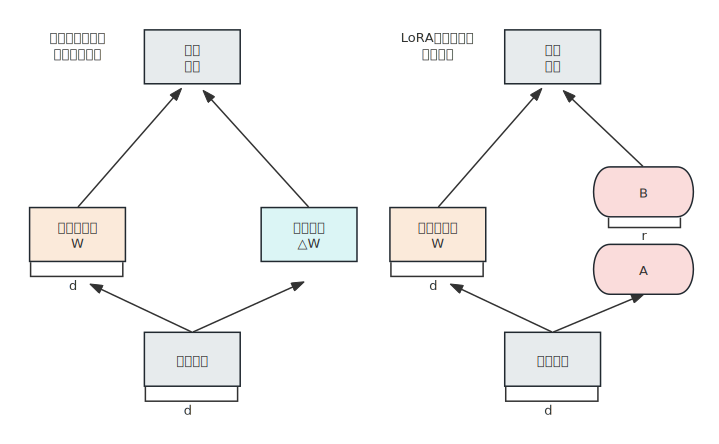
\includegraphics[width=\textwidth]{image/LoRA.pdf}
  \caption{LoRA的原理结构图}
  \label{LoRA}
\end{figure}

P-tuning v2方法是对Deep Prompt Tuning\cite{li2021prefix}\cite{qin2021learning}的一种改进和适应性实现。Fine-tuning方法需要微调整个预训练模型,而且加入了新的参数,在训练过程中需要消耗大量内存,而Prompting方法冻结了预训练模型的所有参数,只通过添加Prompt来预测结果,因此可以在不微调的情况下改变预训练模型的输出,但是容易陷入局部最优的困境。Prompt-tuning(代指一系列Prompt微调方法而非单一方法)把Prompt也加入到微调过程中,此时只对Prompt部分参数进行微调而不改变预训练模型的参数。但是Prompt-tuning在模型大小不足、尤其是模型参数少于100亿时表现不佳,尤其是在一些自然语言理解任务中的推理能力十分有限。

因此Deep Prompt Tuning在此基础上作出了改进,使用Prefix-tuning\cite{li2021prefix}的深层模型来加强模型的推理能力,如图\ref{Deep Prompt Tuning}所示:

\begin{figure}[ht]
  \centering
  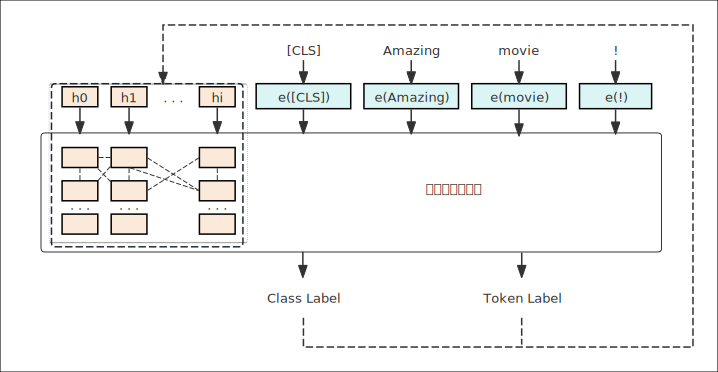
\includegraphics[width=\textwidth]{image/P-tuning v2.pdf}
  \caption{Deep Prompt Tuning的原理结构图}
  \label{Deep Prompt Tuning}
\end{figure}

P-tuning v2就是对Deep Prompt Tuning技术的改进和适应性具体实现,P-tuning v2的优化策略主要包括前缀提示和自适应优化,前者通过将提示信息加入到模型中以提高输出准确性,后者则根据模型在训练中的表现动态调整参数的权重,提高模型微调时的收敛速度。

\subsection{评价指标的选择与介绍}
本文采用目前文本翻译任务最常用的评估指标Bleu系列\cite{papineni2002bleu}中的Bleu-4和Rouge系列\cite{lin2004rouge}中的Rouge-1、Rouge-2、Rouge-L来评价模型。Bleu指标的总体思想就是准确率,是一种基于n-gram模型计算精确度的来评价句子之间相似度的方法,在n-gram下语言模型生成的文本和标准译文的匹配度计算公式如式\ref{n-gram}所示:

\begin{equation}
\label{n-gram}
p_n = \frac{\sum_{c \in \text{candidates}} \sum_{\text{n-gram} \in c} \text{Count}_{\text{clip}}(\text{n-gram})}{\sum_{c' \in \text{candidates}} \sum_{\text{n-gram}' \in c'} \text{Count}_{\text{clip}}(\text{n-gram}')}
\end{equation}

其中,$candidate$表示语言模型生成的文本,$reference$表示标准译文,$Count_{clip}(n-gram)$表示某个$n-gram$在$reference$中的个数,所以分子就是在给定的$candidate$中有多少个$n-gram$出现在$reference$中,分母表示所有的$candidate$中$n-gram$的个数。此时Bleu的最终计算公式为式\ref{bleu}:

\begin{equation}
\label{bleu}
Bleu = BP \times \exp\left(\sum_{n=1}^N w_n \log(p_n)\right)
\end{equation}

其中$BP$是惩罚因子,$w_n$是每个n-gram的权重。Bleu方法根据所使用的n-gram模型的n的取值分为多种评价指标,常见的n指标有1、2、3、4四种。其中Bleu-1衡量的是单词级别的准确性,偏向于较短的翻译结果,越高阶的Bleu方法的评价约倾向衡量句子的流畅度,在文本翻译任务上更要求句子之间语义的相似度和句子的流畅度,而由于文言文和现代文之间文法的巨大差异,单纯衡量单词之间的准确性意义不大,因此我们在Bleu系列指标中仅采用Bleu-4。

Rouge是一种基于召回率的相似度量方法,和Bleu类似,Rouge-N也是基于n-gram模型计算句子的召回率与准确率的比值,衡量模型输出和标准译文之间的相似性,Rouge-N的计算公式和Bleu基本相同,但是是基于召回率的,如式\ref{rouge-n}:

\begin{equation}
\label{rouge-n}
\text{Rouge-N} = \frac{\sum_{c \in \text{references}} \sum_{n\text{-gram} \in c} \text{Count}_{\text{clip}}(n\text{-gram})}{\sum_{c' \in \text{references}} \sum_{n\text{-gram}' \in c'} \text{Count}_{\text{clip}}(n\text{-gram}')}
\end{equation}

其中,$candidate$表示语言模型生成的文本,$reference$表示标准译文,$Count_{clip}(n-gram)$表示某个$n-gram$在$reference$中的个数。相比Bleu更关心输出句子的准确度,Rouge-N指标更关心输出句子的充分性和忠实性。但是由于当N>3时Rouge-N指标的值通常都很小,缺少足够的区分度,因此我们只采用Rouge-1和Rouge-2指标。

Rouge-L的思想和Rouge-N类似,只是Rouge-L使用最长公共子序列(LCS)计算召回率,衡量模型输出对标准译文的覆盖程度,公式如式\ref{rouge-l}:

\begin{equation}
\label{rouge-l}
\text{Rouge-L} = \frac{Count_{\text{max}}(\text{LCS})}{Count(\text{reference})}
\end{equation}

其中分子表示语言模型生成的文本和标准译文之间的最长公共子序列的长度,分母表示标准译文的长度。

此外,考虑到文言文和现代文之间语法、句法、词语的巨大差异,仅仅使用机械的评价指标是不能完全体现模型的差异和翻译结果的优美程度,同时评价文言文-现代文的翻译结果也是一个主观性极强的任务,因此加入人工评测指标进行主观评分的补充。

\subsection{实验环境}
整个项目使用Python编程,项目运行的环境、组件依赖和硬件条件如表\ref{environment}所示:

\begin{table}[h]
\renewcommand\arraystretch{1.5}
\caption{项目运行的环境、组件依赖和硬件条件}
\label{environment}
\begin{tabular}{|l|l|}
\hline
\textbf{项目}     & \textbf{版本号}         \\ \hline
操作系统            & Ubuntu 22.04.2 LTS   \\ \hline
Python版本        & 3.8.19               \\ \hline
Transformers库版本 & 4.28.1               \\ \hline
ModelScope库版本   & 1.13.3               \\ \hline
Pytorch库版本      & 1.13.1+cu117         \\ \hline
cuda版本          & 11.7                 \\ \hline
GPU型号           & Tesla V100-SXM3-32GB \\ \hline
\end{tabular}
\end{table}

\section{实验过程}
\subsection{准备数据}
在微调模型之前,我们要对数据进行预处理,包括数据清洗、格式转换等操作,同时需要将储存在不同文件的文言文语料数据和对应的现代文预料数据转换成文言文-现代文平行语料数据。同时,针对ChatGLM3-6B的训练数据,我们用“请将这段文言文翻译为现代文:”作为Prompt提示。输入数据格式如图\ref{en},数据准备部分的脚本如图\ref{python}:


\begin{figure}[H]
  \centering
  \includegraphics[width=\textwidth]{image/数据格式.png}
  \caption{输入数据格式}
  \label{en}
\end{figure}

\begin{figure}[H]
    \centering
    {\linespread{1.0}
\begin{lstlisting}[   
language=Python, 
style=pycharm,
]
def generate_json_object(id, str1, str2):
    """
    生成一个 JSON 对象
    """
    json_object = {
        "content": "请将这段文言文翻译为现代文:" + str1.replace("请翻译以下文言文语句:", ''),
        "summary": str2
    },
    return json_object

def read_lines(file_path):
    with open(file_path, 'r') as file:
        lines = file.readlines()
    return lines


def main(file1_path, file2_path):
    lines_file1 = read_lines(file1_path)
    lines_file2 = read_lines(file2_path)

    # 确保两个文件中行数相同,否则无法一一对应
    if len(lines_file1) != len(lines_file2):
        print("Error: 文件行数不一致")
        return

    # 输出对应行的数据
    json_objects = []
    for line1, line2 in zip(lines_file1, lines_file2):
        if len(line1.strip()) < 6 or (len(line2.strip()) > len(line1.strip()) * 2):
            print(line1.strip() + ' ' + str(len(line1.strip())))
            continue
        print(line1.strip(), line2.strip())
        # 生成多个 JSON 对象
        json_object = generate_json_object(cnt, line1.strip(), line2.strip())
        json_objects.append(json_object)

    # 将多个 JSON 对象写入文件
    with open("test-all.json", "a") as f:
        json.dump(json_objects, f, indent=2, ensure_ascii=False)
\end{lstlisting}
}
    \caption{数据准备脚本}
    \label{python}
\end{figure}

根据脚本,从Erya数据集中,我们整理出一个20000条数据的的小规模训练集,用于初步验证模型微调脚本的可行性,比较在较少数据情况下模型性能相比未微调的预训练模型的变化。以及一个200000条数据的中等规模训练集、一个500000条数据的正式训练集,其中500000规模数据集完全包括200000规模的训练集,用于比较在训练数据变大以及训练时间增长时模型性能的变化。在训练集以外,我们从评测基准数据集里整理出一个2000条数据的小规模验证集,用于快速验证模型在训练过程中的性能表现,在短时间内获得较为全面的模型性能数据,节省训练资源。以及一个约110000条数据规模的测试集,用于与其他模型做横向对比。针对NiuTrans数据集,根据脚本我们整理出一个500000条数据规模的对照训练集。

\subsection{微调脚本}
微调脚本方面,我们使用THUDM发布的官方工具仓库\footnote{THUDM发布的GitHub代码仓库.\url{https://github.com/THUDM/ChatGLM-6B.git}.},仓库中支持工具调用、代码执行、模型微调等功能,中提供的P-tuning v2微调脚本,脚本参数如图\ref{canshu1}:

\begin{figure}[h]
    \centering
    {\linespread{1.0}
\begin{lstlisting}[   
language=Python, 
style=pycharm,
]
PRE_SEQ_LEN=128
LR=2e-2

CUDA_VISIBLE_DEVICES=1 python3 main.py \
    --do_train \
    --train_file ChatGLM-6B/ptuning/ptuning.json \
    --validation_file ChatGLM-6B/ptuning/valid.json \
    --prompt_column content \
    --response_column summary \
    --overwrite_cache \
    --model_name_or_path ChatGLM-6B/model/ZhipuAI/ChatGLM-6B \
    --output_dir output \
    --overwrite_output_dir \
    --max_source_length 128 \
    --max_target_length 128 \
    --per_device_train_batch_size 8 \
    --per_device_eval_batch_size 1 \
    --gradient_accumulation_steps 2 \
    --predict_with_generate \
    --max_steps 350001 \
    --logging_steps 10 \
    --save_steps 5000 \
    --learning_rate $LR \
    --pre_seq_len $PRE_SEQ_LEN \
    --quantization_bit 4
\end{lstlisting}
}
    \caption{P-tuning v2微调脚本参数}
    \label{canshu1}
\end{figure}

对于LoRA方法,我们使用GitHub仓库\footnote{ChatGLM3-6B的LoRA微调脚本GitHub仓库.\url{https://github.com/hiyouga/ChatGLM-Efficient-Tuning.git}.}中提供的脚本,脚本参数如图\ref{canshu2}:

\begin{figure}
    \centering
    {\linespread{1.0}
\begin{lstlisting}[   
language=Python, 
style=pycharm,
]

CUDA_VISIBLE_DEVICES=0 python train_bash.py \
    --stage sft \
    --model_name_or_path ChatGLM-6B/model/ZhipuAI/ChatGLM-6B \
    --do_train \
    --dataset ancient-trans \
    --finetuning_type lora \
    --output_dir ChatGLM-6B/ChatGLM-Efficient-Tuning-main/output \
    --per_device_train_batch_size 4 \
    --gradient_accumulation_steps 4 \
    --lr_scheduler_type cosine \
    --logging_steps 10 \
    --save_steps 5000 \
    --learning_rate 5e-4 \
    --num_train_epochs 5.0 \
    --plot_loss \
    --fp16
\end{lstlisting}
}
    \caption{LoRA微调脚本参数}
    \label{canshu2}
\end{figure}

\subsection{训练过程}
对于Ptuning-v2微调方法,在使用Erya数据集构建的20000、200000、500000的规模训练集上,模型微调过程loss大致的变化图如图\ref{2w-loss}、\ref{20w-loss}、\ref{50w-loss}所示:

\begin{figure}[H]
  \centering
  \includegraphics[width=0.75\textwidth]{image/2w-loss.png}
  \caption{20000规模数据集微调模型loss变化图}
  \label{2w-loss}
\end{figure}

\begin{figure}[H]
  \centering
  \includegraphics[width=0.75\textwidth]{image/20w-loss.png}
  \caption{200000规模数据集微调模型loss变化图}
  \label{20w-loss}
\end{figure}

\begin{figure}[H]
  \centering
  \includegraphics[width=0.75\textwidth]{image/50w-loss.png}
  \caption{500000规模数据集微调模型loss变化图}
  \label{50w-loss}
\end{figure}

对于LoRA微调方法,在使用Erya数据集构建的500000规模数据集上的loss大致变化如图\ref{50w-lora-loss}所示:

\begin{figure}[h]
  \centering
  \includegraphics[width=0.75\textwidth]{image/50w-lora-loss.png}
  \caption{50000规模数据集的LoRA方法微调模型loss变化图}
  \label{50w-lora-loss}
\end{figure}

对于使用NiuTrans数据集构建的500000规模长文本训练集上的微调,我们也使用P-tuning v2方法进行训练,loss变化如图\ref{50w-long-loss}所示:

\begin{figure}[h]
  \centering
  \includegraphics[width=0.75\textwidth]{image/50w-long-loss.png}
  \caption{50000规模NiuTrans数据集的P-tuning v2方法微调模型loss变化图}
  \label{50w-long-loss}
\end{figure}

可以看到,无论是哪种规模的数据集和微调方法,微调过程中模型的loss变化都是总体呈下降趋势,在图\ref{2w-loss}中可以看出在前几个step中loss下降非常明显,之后loss下降逐渐放缓。而在20000以上的数据集上,模型的loss在下降至2.0-1.8附近时处于波动状态,整体不再趋近于下降,这符合一般大语言模型在微调时的收敛状态,体现出我们对微调参数的选择、模型的训练基本是正确的,模型的训练过程是有效的。

\subsection{验证集表现}
我们首先使用20000、200000、500000规模的数据集,使用P-tuning v2方法对ChatGLM3-6B模型进行初步微调,以验证模型在文言文-现代文翻译任务上的可行性和增大训练集规模对模型性能的影响,针对使用P-tuning v2方法微调,我们对比了不进行微调的ChatGLM3-6B模型、使用20000规模数据集微调、使用200000规模数据集微调、使用500000规模数据集微调在验证集上的表现,在表\ref{score1}中表示为ChatGLM3-6B、ChatGLM3-6B-20000、ChatGLM3-6B-200000、ChatGLM3-6B-500000,其中,ChatGLM3-6B-200000、ChatGLM3-6B-500000在训练过程中的评分变化分别如图\ref{20w-score}、\ref{50w-score}所示:

\begin{table}[h]
\renewcommand\arraystretch{1.5}
\caption{ChatGLM3-6B、ChatGLM3-6B-20000、ChatGLM3-6B-200000、ChatGLM3-6B-500000训练过程的评分}
\label{score1}
\begin{tabular}{|l|l|l|l|l|}
\hline
\textbf{模型/指标}     & \textbf{Bleu-4} & \textbf{Rouge-1} & \textbf{Rouge-2} & \textbf{Rouge-L} \\ \hline
ChatGLM3-6B        & 12.6734         & 31.4470          & 10.8959          & 28.9438          \\ \hline
ChatGLM3-6B-20000  & 25.8668         & 45.4187          & 21.1878          & 45.9646          \\ \hline
ChatGLM3-6B-200000 & 29.2028         & 49.3595          & 24.6433          & 49.8838          \\ \hline
chatGLM3-6B-500000 & 30.4521         & 50.2036          & 26.0271          & 50.7910           \\ \hline
\end{tabular}
\end{table}

\begin{figure}[h]
  \centering
  \includegraphics[width=0.75\textwidth]{image/20w-score.png}
  \caption{ChatGLM3-6B-200000的评分变化图}
  \label{20w-score}
\end{figure}

\begin{figure}[h]
  \centering
  \includegraphics[width=0.75\textwidth]{image/50w-score.png}
  \caption{ChatGLM3-6B-500000的评分变化图}
  \label{50w-score}
\end{figure}

根据表\ref{score1}的数据可以看出,ChatGLM3-6B模型在使用20000数据集简单微调以后,相比未微调预训练模型在各个指标上均有较大提升(+13Bleu),而相比使用20000小数据集微调的效果,使用20000规模数据集进行微调获得的模型在后续训练中表现出更好的性能(+4Bleu),而继续增加数据集规模的chatGLM3-6B-500000在验证集上的性能也取得了增长(+2.4Bleu)。随着训练数据集规模的增长,Rouge分数也均有较高增长,说明模型的输出文本相比标准译文的准确度、流畅度都有提升。实验结果表明,在基线模型的基础上注入大量文言文-现代文语料数据进行训练,能够有效提升模型对文言文的理解和推理能力。此外,随着微调语料规模的增加,模型处理下游任务知识的能力也在逐步增强。

由于不同的微调方法各有优势,我们分别使用P-tuning v2方法、LoRA方法在相同的数据集上对ChatGLM3-6B进行微调,以验证不同的微调方法的影响,在表\ref{pt-lora}中表现为ChatGLM3-6B-P-tuning v2、ChatGLM3-6B-LoRA:

\begin{table}[]
\renewcommand\arraystretch{1.5}
\caption{ChatGLM3-6B-P-tuning v2、ChatGLM3-6B-LoRA在验证集上的分数}
\label{pt-lora}
\begin{tabular}{|l|l|l|l|l|}
\hline
\textbf{模型/指标}          & \textbf{Bleu-4} & \textbf{Rouge-1} & \textbf{Rouge-2} & \textbf{Rouge-L} \\ \hline
ChatGLM3-6B-P-tuning v2 & 30.4521         & 50.2036          & 26.0271          & 50.7910           \\ \hline
ChatGLM3-6B-LoRA        & 26.9438         & 46.8453          & 22.7816          & 47.4667          \\ \hline
\end{tabular}
\end{table}

使用P-tuning v2方法微调模型在Bleu和Rouge指标上均比使用LoRA微调模型的分数要高(+4.7Bleu),这验证了使用P-tuning v2方法进行微调的正确性。

由于文言文-现代文平行语料库在作为模型的训练数据时,不同数据类型、文本长度、文言文来源年代、数据来源语料库等变量都可能会影响模型的性能,我们分别使用Erya数据集和NiuTrans数据集构建了相同大小的训练集,并使用P-tuning v2方法训练了相同的时间,在表\ref{E-N}中表现为ChatGLM3-6B-Erya、ChatGLM3-6B-NiuTrans:

\begin{table}[]
\renewcommand\arraystretch{1.5}
\caption{ChatGLM3-6B-Erya、ChatGLM3-6B-NiuTrans在验证集上的分数}
\label{E-N}
\begin{tabular}{|l|l|l|l|l|}
\hline
\textbf{模型/指标}       & \textbf{Bleu-4} & \textbf{Rouge-1} & \textbf{Rouge-2} & \textbf{Rouge-L} \\ \hline
ChatGLM3-6B-Erya     & 30.4521         & 50.2036          & 26.0271          & 50.7910           \\ \hline
ChatGLM3-6B-NiuTrans & 26.8861         & 46.2848          & 22.3509          & 46.2564          \\ \hline
\end{tabular}
\end{table}

相比Erya数据集,NiuTrans数据集的文言文-现代文数据的单条数据长度更长、文言文来源更广更杂更早,因此在模型上进行训练的结果也不同,使用Erya数据集训练的结果相比使用NiuTrans数据集的结果取得了+4.8Bleu、平均+5Rouge的差距,这验证了选择Erya训练集的正确性。

\section{本章小结}
在这一章中,从项目规划、实验过程两个方面介绍了我们的项目,首先介绍了项目进行的规划,包括数据集的构建、模型的选择、评价指标的选择等,分析了项目的前期工作。然后阐述了项目的具体实验过程,介绍了项目所使用的脚本和代码仓库,展示了模型在训练过程中的变化和趋势,并对比了经过训练获得的模型在验证集上的表现,证明了模型的微调方法是正确且有效的。

\chapter{实验结果及分析}
\section{基线对比模型选择}
\subsection{百度翻译}
百度翻译是百度旗下的新一代AI大模型企业翻译平台,我们调用百度翻译提供的通用文本翻译API,将源语言设置为“wyw”、目的语言设置为“zh”进行调用,调用脚本如图\ref{baidu-api}所示:

\begin{figure}[h]
    \centering
    {\linespread{1.0} % 设置行间距
    \begin{lstlisting}[   
    language=Python, 
    style=pycharm,
    ]
def main(text):
    url = "https://aip.baidubce.com/rpc/2.0/mt/texttrans/v1?access_token=" + get_access_token()
    ans = []
    for str1 in text:
        payload = json.dumps({
            "from": "wyw",
            "to": "zh",
            "q": str1,
        })
        headers = {
            'Content-Type': 'application/json',
            'Accept': 'application/json'
        }

        response = requests.request("POST", url, headers=headers, data=payload)
        ans.append(response.text)
        print(response.text)
    return ans

def get_access_token():
    """
    使用 AK,SK 生成鉴权签名(Access Token)
    :return: access_token,或是None(如果错误)
    """
    url = "https://aip.baidubce.com/oauth/2.0/token"
    params = {"grant_type": "client_credentials", "client_id": API_KEY, "client_secret": SECRET_KEY}
    return str(requests.post(url, params=params).json().get("access_token"))
    
    \end{lstlisting}
    }
    \caption{百度翻译API调用脚本}
    \label{baidu-api}
\end{figure}

\subsection{【随无涯】翻译模型}
 【随无涯】是一个huggingface spaces + streamlit 的古文阅读应用(含海量书籍),其作者在hugging face上发布了这个应用的源翻译模型【raynardj/wenyanwen-ancient-translate-to-modern】\footnote{【随无涯】的源模型的Hugging Face主页.\url{https://huggingface.co/spaces/raynardj/duguwen-classical-chinese-to-morden-translate}.},我们选择使用这个模型作为对比基线模型,使用作者推荐的运行参数在测试集上运行,参数及调用脚本如图\ref{wyw-run}所示:
 
\begin{figure}[h]
    \centering
{\linespread{1.0}
\begin{lstlisting}[   
language=Python, 
style=pycharm,
]
def inference(text):
    tk_kwargs = dict(
      truncation=True,
      max_length=128,
      padding="max_length",
      return_tensors='pt')
   
    inputs = tokenizer([text,],**tk_kwargs)
    with torch.no_grad():
        return tokenizer.batch_decode(
            model.generate(
            inputs.input_ids,
            attention_mask=inputs.attention_mask,
            num_beams=3,
            max_length=256,
            bos_token_id=101,
            eos_token_id=tokenizer.sep_token_id,
            pad_token_id=tokenizer.pad_token_id,
        ), skip_special_tokens=True)
\end{lstlisting}
}
    \caption{【随无涯】运行参数}
    \label{wyw-run}
\end{figure}

\subsection{mengzi-t5-base}
T5模型作为一个经典的预训练模型,被广泛的用来作为各种论文中的基线对比模型,然而原本由谷歌发布的T5预训练模型在中文语料下的表现不尽如人意,因此我们选择了澜舟科技(Langboat)发布的孟子系列预训练模型中的mengzi-t5-base\cite{zhang2021mengzi},即孟子中文T5预训练模型。mengzi-t5-base生成模型与T5结构相同,不包含下游任务,只有无监督数据训练。因此我们将mengzi-t5-base在与ChatGLM3-6B相同的训练集上进行微调,使用微调后的模型作为基线对比模型,微调参数如图\ref{megnzi}所示:

\begin{figure}
    \centering
    {\linespread{1.0}
\begin{lstlisting}[   
language=Python,
style=pycharm,
]
model_params = {
    "MODEL": "/home/wbw/T5/model/Langboat:mengzi-t5-base",  # model_type: t5-base/t5-large
    "TRAIN_BATCH_SIZE": 8,  # training batch size
    "TRAIN_EPOCHS": 5,  # number of training epochs
    "LEARNING_RATE": 1e-4,  # learning rate
    "MAX_SOURCE_TEXT_LENGTH": 128,  # max length of source text
    "MAX_TARGET_TEXT_LENGTH": 128,  # max length of target text
    "SEED": 42,  # set seed for reproducibility
  }
\end{lstlisting}
}
    \caption{mengzi-t5-base微调参数}
    \label{megnzi}
\end{figure}

\subsection{Qwen1.5-1.8B}
使用通义千问发布的Qwen1.5-1.8B模型进行微调作为基线模型\footnote{Qwen1.5-1.8B的源模型的Model Scope主页.\url{https://modelscope.cn/models/qwen/Qwen1.5-1.8B/summary}.},使用相同的训练集和LoRA方法进行微调\footnote{Qwen1.5-1.8B的微调脚本的GitHub仓库.\url{https://github.com/QwenLM/Qwen}.},微调脚本如图\ref{qwen-finetune}所示:

\begin{figure}
    \centering
    {\linespread{1.0}
\begin{lstlisting}[   
language=Python,
style=pycharm,
]
python finetune.py \
  --model_name_or_path $MODEL \
  --data_path $DATA \
  --bf16 True \
  --output_dir output_qwen \
  --num_train_epochs 5 \
  --per_device_train_batch_size 2 \
  --per_device_eval_batch_size 1 \
  --gradient_accumulation_steps 8 \
  --evaluation_strategy "no" \
  --save_strategy "steps" \
  --save_steps 1000 \
  --save_total_limit 10 \
  --learning_rate 3e-4 \
  --weight_decay 0.1 \
  --adam_beta2 0.95 \
  --warmup_ratio 0.01 \
  --lr_scheduler_type "cosine" \
  --logging_steps 1 \
  --report_to "none" \
  --model_max_length 512 \
  --lazy_preprocess True \

  --gradient_checkpointing \
  --use_lora

\end{lstlisting}
}
    \caption{Qwen1.5-1.8B的微调脚本}
    \label{qwen-finetune}
\end{figure}

\section{超参数的选择}
ChatGLM3-6B模型在执行生成任务时的参数主要有$Top_p$、$Top_k$、$Temperature$三个,模型在生成输出序列,会根据根据输入序列来预测输出的每一个token,每次模型都会生成一个可能的token概率分布列表,表示模型对后续的token预测的概率,预测过程如图\ref{yu ce}所示。

\begin{figure}[ht]
  \centering
  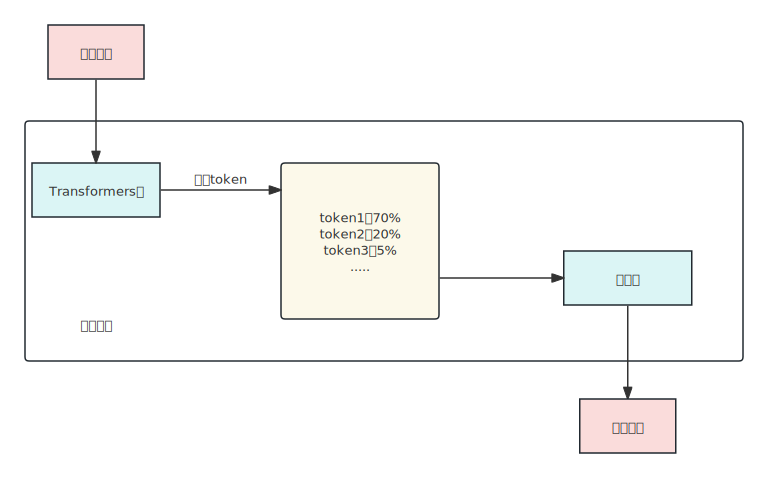
\includegraphics[width=\textwidth]{image/预测token.pdf}
  \caption{ChatGLM3-6B选择Token的过程}
  \label{yu ce}
\end{figure}

在选择token的过程中,模型会根据采样策略选择不同的token,而调整采样策略就可以对模型输出的多样性、准确性和质量进行调控,以满足不同的需求和场景。而参数$Top_k$、$Top_p$、$Temperature$可以影响模型采样的策略进而影响模型的输出,$Top_k$采样是一种基于动态词汇集的采样方法,使用$Top_k$采样的模型会从概率排名前k的token集合中进行选择,这样允许其他概率比较高但是并非最高的token也有机会被选中,增大了token选择的随机性和变化性,在很多情况下,$Top_k$抽样带来的随机性有助于提高生成质量。

$Top_p$采样与$Top_k$相似,在每一步,$Top-p$采样仅从累积概率超过阈值p的最小token集合中进行随机采样,忽略其他低概率的token。这种方法聚焦于概率分布的核心部分,而忽略了尾部部分,以避免采样到不合适或不相关的单词。这样一来,模型能够保留一些有趣或有创意的单词,使得生成结果更具吸引力和相关性。$Top_p$策略通常和$Top_k$策略一起使用,模型会在这两种策略中较小的那个token集合中进行采样。$Top_k$和$Top_p$的值越低,则模型生成的输出越稳定,但是会导致结果十分无聊,在文言文-现代文翻译任务中,可能会使输出译文过于死板,失去文本在文学上的流畅度,降低阅读体验。而$Top_k$、$Top_p$设置的值过高,模型的输出会趋近去随机,虽然这样能提高输出和随机性但是有可能会大幅度降低准确性,失去文本应有的语义,降低输出译文的质量。

$Temperature$采样是用于调节Softmax函数输出分布的参数。在生成文本时,Softmax函数将模型输出转换为概率分布,用于选择下一个词汇。通过调节$Temperature$参数,可以改变 Softmax 函数的输出分布的“平缓程度”。较高的$Temperature$值会使得概率分布更平滑,输出的token概率之间的方差越小,从而生成的文本更加多样化;而较低的$Temperature$值会使得概率分布更集中,生成的文本更加保守。

ChatGLM3-6B的代码实现的应用场景为聊天机器人,而聊天机器人要求模型的输出文本应当有足够的随机性和趣味性,因此在其代码中超参数的默认取值为$Top_p$=0.7、$Temperature$=0.95、不设置$Top_k$。在文言文-现代文翻译任务上需要模型输出保持一定的质量和准确性,如此高的采样概率显然是没必要的,因此我们针对超参数在验证集上进行对比实验,通过按顺序调整$Top_k$、$Temperature$、$Top_p$来尝试获得最好的生成效果下的参数,实验结果如表\ref{scorecanshu}、单个参数的分数变化图如\ref{topp}、\ref{temp}、\ref{topk}所示:

\begin{table}[]
\renewcommand\arraystretch{1.5} % 设置表格行高
\caption{不同的超参数在验证集上的分数}
\label{scorecanshu}
\begin{tabular}{|l|l|l|l|l|}
\hline
\textbf{参数设置/指标}                       & \textbf{Bleu-4} & \textbf{rouge-1} & \textbf{rouge-2}   & \textbf{rouge-l} \\ \hline
Top\_p=0.7,Temperature=0.95,未设置Top\_k  & 30.4521         & 50.2036          & 26.0271            & 50.791           \\ \hline
Top\_p=0.40,Temperature=0.95,未设置Top\_k & 30.8018         & 50.8867          & 26.617             & 51.4093          \\ \hline
Top\_p=0.35,Temperature=0.95,未设置Top\_k & \textbf{30.8327}         & \textbf{50.8768}          & \textbf{26.4786}            & \textbf{51.4007}          \\ \hline
Top\_p=0.20,Temperature=0.95,未设置Top\_k & 30.0231         & 50.1054          & 25.9861            & 50.1063          \\ \hline
Top\_p=0.35,Temperature=0.60,未设置Top\_k & 31.645          & 51.6325          & 27.3558            & 52.2489          \\ \hline
Top\_p=0.35,Temperature=0.50,未设置Top\_k & 31.5085         & 51.617           & 27.2271            & 52.2474          \\ \hline
Top\_p=0.35,Temperature=0.01,未设置Top\_k & \textbf{31.5728}      & \textbf{51.7012}       & \textbf{27.2839} & \textbf{52.3049}      \\ \hline
Top\_p=0.35,Temperature=0.60,Top\_k=5  & 31.3918         & 51.5079          & 27.1022            & 52.1111          \\ \hline
Top\_p=0.35,Temperature=0.60,Top\_k=3  & 31.7543         & 51.8071          & 27.4401            & 52.3731          \\ \hline
Top\_p=0.35,Temperature=0.60,Top\_k=2  & 31.2762         & 51.2558          & 27.0408            & 52.0612          \\ \hline
Top\_p=0.35,Temperature=0.55,Top\_k=3  & 31.7561         & 51.7932          & 27.426             & 52.3624          \\ \hline
Top\_p=0.35,Temperature=0.50,Top\_k=3  & \textbf{31.7664}         & \textbf{51.7983}          & \textbf{27.4502}            & \textbf{52.3663}          \\ \hline
\end{tabular}
\end{table}

\begin{figure}[H]
  \centering
  \includegraphics[width=0.75\textwidth]{image/Top-p-score.png}
  \caption{$Temperature=0.95$,未设置$Top_k$时评分随$Top_p$取值变化}
  \label{topp}
\end{figure}

\begin{figure}[H]
  \centering
  \includegraphics[width=0.75\textwidth]{image/Temperature-score.png}
  \caption{$TOP_p=0.35$,未设置$Top_k$时评分随$Temperature$取值变化}
  \label{temp}
\end{figure}

\begin{figure}[H]
  \centering
  \includegraphics[width=0.75\textwidth]{image/Top-k-score.png}
  \caption{$TOP_p=0.35$,$Temperature=0.95$,评分随$Top_k$取值变化}
  \label{topk}
\end{figure}

经过实验,发现$Top_p=0.35$、$Temperature=0.50$、$Top_k=3$的最终评分最高,在后续的对比实验中也将对ChatGLM3-6B使用$Top_p=0.35$、$Temperature=0.50$、$Top_k=3$的超参数进行实验。

\section{对比实验}

\subsection{测试集对比实验}
在测试集上,(1)对比百度翻译,由于百度API的限额要求,因此无法翻译整个测试集,因此对百度翻译我们尽可能多的在测试集上翻译了6000余条,使用这6000条数据作为百度翻译的测试集。(2)对于【随无涯】翻译模型,我们使用作者推荐的超参数进行生成。(3)对于mengzi-t5-base,使用进行微调后的模型进行生成。(4)对于Qwen1.5-1.8B,使用LoRA方法进行微调后生成。实验结果如表\ref{baidu-caht}、\ref{mengzi-wyw-caht}所示:

\begin{table}[h]
\renewcommand\arraystretch{1.5}
\caption{百度翻译与ChatGLM3-6B在测试集上的分数对比}
\label{baidu-caht}
\begin{tabular}{|l|l|l|l|l|}
\hline
\textbf{模型/指标} & \textbf{Bleu-4} & \textbf{rouge-1} & \textbf{rouge-2} & \textbf{rouge-l} \\ \hline
百度翻译           & 29.6460         & 49.4751          & 22.7385          & 50.1843          \\ \hline
ChatGLM3-6B    & 29.8697         & 54.1254          & 29.4477          & 54.8262          \\ \hline
\end{tabular}
\end{table}

\begin{table}[h]
\renewcommand\arraystretch{1.5}
\caption{【随无涯】、mengzi-t5-base与ChatGLM3-6B在测试集上的分数对比}
\label{mengzi-wyw-caht}
\begin{tabular}{|l|l|l|l|l|}
\hline
\textbf{模型/指标} & \textbf{Bleu-4} & \textbf{rouge-1} & \textbf{rouge-2} & \textbf{rouge-l} \\ \hline
【随无涯】翻译模型      & 26.1356         & 48.3732          & 18.7722          & 47.8400          \\ \hline
chatGLM3-6B    & 33.7967         & 56.0598          & 30.8991          & 55.8341          \\ \hline
mengzi-t5-base & 30.9193         & 55.5103          & 38.0098          & 55.0582          \\ \hline
Qwen1.5-1.8B & 19.5024         & 49.5578          & 26.8344          & 49.0509          \\ \hline
\end{tabular}
\end{table}

微调后的模型比所有基线模型都具有更好的翻译能力,与百度翻译相比,Bleu指标上分数接近,在Rouge分数上取得较高的分数(平均+5Rouge);与【随无涯】翻译模型相比,在Bleu和Rouge分数上取得了很大的优势(+7Bleu、平均+10Rouge);与mengzi-t5-base相比,在Bleu-4和Rouge-2上有较大优势(+3Bleu、+8Rouge-2),在Rouge-1和Rouge-L指标上也有轻微优势;与Qwen1.5-1.8B相比的优势也十分明显(+14Bleu、平均+6Rouge)。

\subsection{人工评分对比实验}
在翻译领域,大语言模型的性能评估不能仅仅依赖于数据指标评分,Bleu和Rouge指标无法完全捕捉语义准确性、流畅性和文化特征等与翻译质量相关的方面,进行主观的人的评分是至关重要的。人类评分者可以更好地理解翻译的上下文和意图,能够判断翻译是否符合特定场景的语言习惯和文化背景。他们的主观评价可以提供有价值的反馈,帮助进一步改进和优化大语言模型在翻译任务中的表现。因此,针对人工评分对比实验,我们邀请了6位在文学领域有一定造诣的同学作为评分者,选取了184条记录,对百度翻译、chatGLM3-6B、【随无涯】翻译模型输出的结果进行人工打分。我们从三个方面来考虑生成文本的质量:信(翻译文本与古代文本在语义上是否准确)、达(翻译文本是否流畅和清晰)、雅(翻译文本是否适当和文雅),对每条数据记录在0分到5分的范围内进行打分,其中5分表示“非常满意”,0分表示“非常糟糕”。人工评分结果如表\ref{rengong}所示:

\begin{table}[]
\renewcommand\arraystretch{1.5}
\caption{百度翻译、【随无涯】与ChatGLM3-6B的人工评分对比}
\label{rengong}
\begin{tabular}{|l|l|l|l|l|l|l|}
\hline
\textbf{模型/得分} & \textbf{评分者1} & \textbf{评分者2} & \textbf{评分者3} & \textbf{评分者4} & \textbf{评分者5} & \textbf{评分者6} \\ \hline
百度翻译           & 2.83          & 2.73          & 3.49          & 3.02          & 3.15          & \textbf{3.14} \\ \hline
【随无涯】翻译模型      & 2.84          & 2.20          & \textbf{3.61} & 2.73          & 3.29          & 2.85          \\ \hline
chatGLM3-6B    & \textbf{3.72} & \textbf{3.36} & 3.43          & \textbf{3.81} & \textbf{3.45} & 2.92          \\ \hline
\end{tabular}
\end{table}

人工评分结果中,有4位评分者给我们训练后的模型打出最高分,另外两位评分者的评分中,我们的模型和其他基线模型的得分也很接近,这证明了基于ChatGLM3-6B训练后的模型的优势。

\section{本章小结}
本章介绍了在对ChatGLM3-6B进行微调训练后的对比实验,首先说明了作为基线的对比模型的选择,分别选择了一个商业模型、一个应用模型、两个预训练模型作为对比。然后,介绍了在实验中使用的ChatGLM3-6B模型的生成代码中超参数的对比实验,分析超参数的不同选择在验证集上的不同表现。最后,我们对ChatGLM3-6B和基线模型进行了对比实验,验证了训练后模型在文言文-现代翻译任务中的优势,证明了基线模型选择和构建高效数据集的正确性。

\chapter{总结与展望}
在本论文中,我们针对文言文-现代文翻译任务,使用了P-tuning v2方法对ChatGLM3-6B模型进行微调,并在构建的文言文-现代文平行语料数据集上进行了实验。我们首先对现在的大语言模型研究背景和发展现状做了介绍,然后分析了目前国内外的主流预训练模型,之后对设计的微调实验进行了详细的规划和介绍,包括数据集构建、基础模型选择、微调方法介绍与选择、评价指标的选择与介绍以及实验环境的搭建。随后,我们描述了实验过程,包括数据准备、微调脚本、训练过程以及验证集表现。最终与基线模型进行了对比实验,我们的模型在测试集和人工评分方面均取得了较高的评分。

根据实验结果,我们可以证明:

\begin{itemize}
    \item P-tuning v2方法对ChatGLM3-6B模型进行微调在文言文-现代文翻译任务中取得了显著的性能提升。
    \item 基于Erya数据集构建的训练数据集在模型微调任务中具有较好的质量。
    \item 在各项对比实验中,微调后的ChatGLM3-6B模型表现出了优异的翻译质量和性能。
    \item 微调后的模型在人工评分实验中也取得了令人满意的结果,显示出了其翻译结果在人类阅读方面的优势。
\end{itemize}

虽然本文最终获得的模型取得了较高的评分,但是仍存在许许多多改进的地方,下面从模型选择、数据集构建、对比实验等方面进行分析,以便为后续研究做一些展望和引导:

\begin{itemize}
    \item 模型选择方面:虽然ChatGLM3-6B预训练模型具有较好性能,但是受限于模型本身参数规模和可用的硬件资源,在实验中只进行了6B参数规模的预训练模型进行微调,未来希望可以在更大规模的预训练模型上进行实验,以尝试获得更好性能的模型。
    \item 数据集构建方面:Erya数据集虽然在一定范围内具有较好的性能,但是中国的文言文古籍何其广阔,文言文语法和句式又何其复杂,我们构建的数据集只能包括一些较为成熟、稳定的文言文语料数据,训练后的模型在与训练集语法类似的古文时性能尚可。但是一旦面对一些古老而难以阅读的文言文翻译任务时,模型的表现则未可知。因此希望能够继续扩大数据集,加入一些更古老、更复杂的文言文语料数据。
    \item 对比实验方面:在翻译领域展现出优异表现的模型数不胜数,虽然挑选的三个翻译模型有一定代表性,但是仍不能全面体现我们的模型的优势。同时对比实验的测试集也是基于较为稳定、成熟的文言文古籍的,不能体现模型在更复杂的文言文上的性能。未来可以增加更多的对比模型,并充实对比实验的测试集,加入更多、更全面的文言文数据。
\end{itemize}

通过持续的研究和实践,我们相信微调技术在大语言模型领域的应用将会不断取得突破性进展,为机器翻译领域的发展贡献更多的力量。
 
%---------------------------------------------------------------------
%	参考文献
%---------------------------------------------------------------------

% 生成参考文献页
\printbibliography

%---------------------------------------------------------------------
%	致谢
%---------------------------------------------------------------------

\begin{acknowledgement}
首先要感谢我的毕业设计的指导老师葛季栋老师,在开题、论文修改等方面给了我许多指导和帮助,我的毕业设计的完成离不开葛季栋老师的悉心指导。

其次要感谢软件学院的余彰恒学长,在我做实验的时候给了我许多指导和帮助,使我懂得如何去推进我的实验和计划。

其次,我要向我的组员、朋友、同学们表示感谢,感谢他们在日常生活学习中给予我的帮助。

感谢我的辅导员宋抟老师、张一品老师,感谢你们在我本科期间对我的关怀和指导,没有你们的关心、支持和帮助就没有我现在的成绩。

我要向我的家人表示感谢,感谢在普通的每一天所给予我的肯定和支持,感谢你们的支持和鼓励让我在学业和生活上都有所成长。

最后,感谢南京大学软件学院对我的培养和教育,让我度过了难忘的本科四年生活!
\end{acknowledgement}

% 完工
\end{document}
